\documentclass{article}

\title{Assignment Computer CZ4003 \\ Lab 2}
\date{2019 \\ November}
\author{Koch Philipp Frederik Edward, N1903454H}

\linespread{1.5}

\usepackage{graphicx}
\usepackage{listings}
\usepackage{color}


\definecolor{orange}{rgb}{0.9531,0.39, 0.14}
\definecolor{gray}{rgb}{0.5,0.5,0.5}
\definecolor{green}{rgb}{0,0.6,0}

\lstset{
	basicstyle=\tiny,
	language=Prolog,
	numbers=left,
	numberstyle=\tiny\color{gray},
	keywordstyle=\color{blue},
	commentstyle=\color{orange},
	stringstyle=\color{green},
	lineskip={-1.5pt},
	breaklines=true,
	breakatwhitespace=true,
	frame=single
}

\begin{document}
	
	\maketitle
	
	\section{Edge Detection}
	\section{Line Finding using Hough Transform}
	\section{3D Stereo}
	\subsection{a)} 
	By using the \textit{conv2} and \textit{rot90} functions, for loops could largely be dispensed with. 
	
	\lstinputlisting[title=Core of the dispfunc Function, firstline=34, lastline=49]{dispfunc.m}
	
	\subsection{b) \& c)}
	Figure 1 shows the distance in the corridor in color. It becomes darker as the distance increases. 
	The intensity in the dispersion map increases as the distance between the similar sections increases with distance. This also increases the distance between the optimal SSD values and therefore the distant surface appears darker.Figure 2 shows the view before the calculation.
	\begin{figure}
		\center
		\caption{Disparity map of the corridor}
		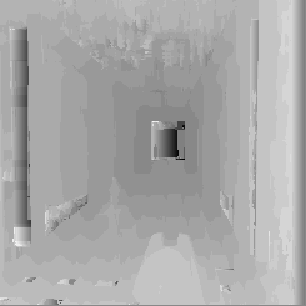
\includegraphics{corridor_disp.png}
		
	\end{figure}
	\begin{figure}
		\center
		\caption{Stereo view before the calculation}
		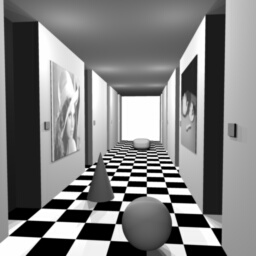
\includegraphics[scale=0.4]{corridorl.jpg}
		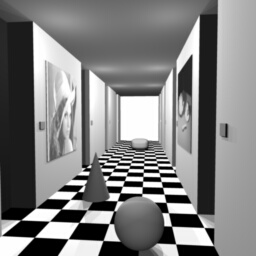
\includegraphics[scale=0.4]{corridorr.jpg}
	\end{figure}
	
	\subsection{d)}
	The result of the next image is different. There is no simple perspective depth in the image. Therefore, the rear part of the image is generally further away, while the front objects are closer. This was shown correctly by the function.
	\begin{figure}
		\center
		\caption{Disparity map of the }
		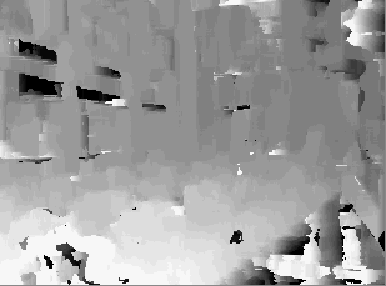
\includegraphics{triclopsi_disp.png}
	\end{figure}
		\begin{figure}
		\center
		\caption{Stereo view before the calculation}
		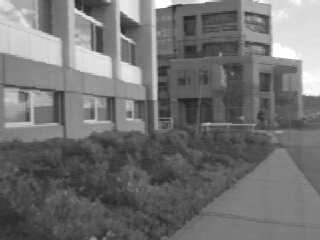
\includegraphics[scale=0.4]{triclopsi2l.jpg}
		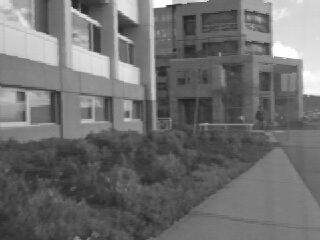
\includegraphics[scale=0.4]{triclopsi2r.jpg}
	\end{figure}
	
\end{document}